\documentclass[12pt]{article}
\usepackage{sbc-template}
\usepackage[utf8]{inputenc}
\usepackage[T1]{fontenc}
\renewcommand{\refname}{Referências}
\renewcommand{\tablename}{Tabela}
\renewcommand{\figurename}{Figura}
\usepackage{graphicx,url,amsmath,amssymb,booktabs,array}
\usepackage[hidelinks]{hyperref}
\sloppy
\title{Priorização de Testes Automatizados sob Restrição de Tempo: uma Avaliação de Heurísticas Gulosas}
\author{Andrey Lourival Andrade Garcia\inst{1}, Igor Cecim Vilhena\inst{2}}
\address{Centro Universitário do Estado do Pará (CESUPA)\\
  Análise e Projeto de Algoritmos -- Belém, PA, Brasil
\nextinstitute
  Centro Universitário do Estado do Pará (CESUPA)\\
  Análise e Projeto de Algoritmos -- Belém, PA, Brasil}
\begin{document}
\maketitle
\begin{abstract}
Automated test prioritization aims to detect faults earlier while retaining the complete test suite. This study compares six ordering strategies in a controlled Python prototype for order processing: reference order, random order, shortest test first, total coverage, additional coverage, and additional coverage per unit of cost. The experiment uses 567 generated cases, 18 individually seeded faults, five suite sizes, and ten repetitions per configuration. Coverage, test duration, prioritization time, and fault detection are measured through actual executions. Ordering metrics are subsequently calculated using an additive model of measured test costs. For 320 tests, the cost-aware heuristic reaches a mean APFDc of 0.9850, close to the 0.9844 obtained by shortest test first. However, its median prioritization time is 60.75 milliseconds, exceeding the execution cost of these short suites. The results connect quadratic greedy work to measured growth and show why prioritization overhead must be evaluated separately from ordering effectiveness. Conclusions are limited to this small artificial benchmark and do not establish superiority on industrial systems.
\end{abstract}
\begin{resumo}
A priorização de testes automatizados procura antecipar a detecção de defeitos preservando a suíte completa. Este estudo compara seis estratégias em um protótipo controlado de processamento de pedidos em Python: ordem de referência, aleatória, menor duração, cobertura total, cobertura adicional e cobertura adicional por unidade de custo. O experimento utiliza 567 casos gerados, 18 defeitos inseridos individualmente, cinco tamanhos de suíte e dez repetições por configuração. Cobertura, duração, tempo de priorização e detecção são obtidos por execuções reais. As métricas das ordenações são calculadas posteriormente por um modelo aditivo dos custos medidos. Para 320 testes, o guloso sensível ao custo alcança APFDc médio de 0,9850, próximo do valor 0,9844 da ordenação por duração. Entretanto, seu tempo mediano de priorização é 60,75 milissegundos, superior ao custo de execução dessas suítes curtas. Os resultados relacionam o trabalho quadrático dos gulosos ao crescimento observado e evidenciam a necessidade de contabilizar o custo da ordenação. As conclusões se restringem ao pequeno ambiente artificial estudado.
\end{resumo}
\noindent\textbf{Palavras-chave:} priorização de testes; algoritmos gulosos; análise de complexidade; APFDc; testes de regressão.
\section{Introdução}
Uma suíte automatizada pode conter testes com durações e capacidades de detecção diferentes. Quando o tempo disponível é limitado, a posição de cada teste influencia o momento em que um defeito se torna observável. A priorização procura uma permutação favorável da suíte, mantendo seus elementos. Essa formulação e a comparação de critérios de cobertura aparecem em \cite{R01}. Seleção, minimização e priorização constituem problemas distintos, também examinados em contexto industrial por \cite{R06}.

Este trabalho adota o eixo E5, algoritmos gulosos, com apoio do eixo E1, análise de complexidade. Seu objetivo é comparar heurísticas simples quanto à antecipação da detecção e ao trabalho computacional necessário para produzir a ordem. O objeto é o MiniPedidos, um protótipo controlado de desconto, frete, estoque e fechamento de pedidos. Sua pequena escala permite inspecionar o procedimento, mas limita a transferência dos resultados para aplicações reais.

As perguntas de pesquisa são: \textbf{QP1}, como as estratégias diferem em detecção antecipada quando os testes têm durações distintas? \textbf{QP2}, o crescimento do custo dos priorizadores acompanha a análise assintótica? \textbf{QP3}, o benefício persiste quando se inclui o tempo de calcular a ordem? A contribuição é um protocolo reproduzível e uma análise de seus compromissos, sem reivindicar um algoritmo novo.
\section{Fundamentação teórica e trabalhos relacionados}
O critério total privilegia testes que cobrem muitos elementos. O adicional considera somente elementos ainda não cobertos na rodada corrente. \cite{R04} analisam estratégias gulosas e de busca e mostram que objetivos diferentes podem favorecer ordens distintas. A comparação é pertinente para E5, mas antecipar cobertura não garante antecipar defeitos.

O trabalho de \cite{R07} estabelece o limite harmônico $H(d)$ para o custo de uma cobertura de conjuntos obtida por escolha gulosa, com $d$ igual ao maior tamanho de um conjunto. A razão entre novos elementos e custo inspira uma das heurísticas deste trabalho. A garantia refere-se à cobertura de custo mínimo; ela não é reivindicada para APFD, APFDc ou para a permutação completa aqui produzida.

\cite{R02} incorporam custos e severidades à avaliação de priorização, enquanto \cite{R05} exploram uma abordagem genética sensível ao tempo. A revisão de \cite{R10} organiza métodos e métricas que consideram custo e valor. Neste projeto, a severidade é uniforme: não existem dados que permitam atribuir pesos realistas aos defeitos artificiais.

Entre os trabalhos recentes, \cite{R08} reduzem o esforço do guloso adicional por aceleração e \cite{R09} investigam atenção parcial. Ambos delimitam alternativas relevantes, mas a reprodução de aprendizado ou de AGA ampliaria o recorte. A comparação implementada utiliza critérios transparentes, cuja execução pode ser contada diretamente. A Tabela~\ref{tab:rel} sintetiza diferenças que orientam o protocolo.

\begin{table}[ht]
\centering\caption{Comparação crítica das linhas de trabalho selecionadas.}\label{tab:rel}
\small
\begin{tabular}{p{2.7cm}p{4.4cm}p{6.3cm}}\toprule
Referência & Foco & Consequência para este projeto\\\midrule
Li et al. (2007) & Gulosos e busca por cobertura & Comparar total e adicional, sem tratar cobertura como detecção.\\
Walcott et al. (2006) & Tempo e busca genética & Medir orçamento temporal, sem reproduzir o método genético.\\
Li et al. (2022) & Aceleração do adicional & Contabilizar o custo da própria priorização.\\
Zhang et al. (2022) & Atenção parcial & Reconhecer alternativas recentes fora do recorte.\\
Inozemtseva e Holmes (2014) & Cobertura e eficácia & Avaliar detecção separadamente.\\\bottomrule
\end{tabular}
\end{table}

A família de estudos de \cite{R03} situa a investigação empírica de priorização. \cite{R11} observam que a relação entre cobertura e eficácia enfraquece ao controlar o tamanho das suítes. \cite{R12} estudam a relação entre mutantes e defeitos reais, mas sua evidência não transforma qualquer conjunto artificial em substituto universal de falhas naturais. Por isso, o protocolo mantém fixos os testes de cada comparação e explicita a origem dos defeitos.

A lacuna adotada é local e didática: verificar se o benefício de reordenar funções muito curtas compensa o custo do priorizador. Os resultados de outros sistemas não resolvem essa questão para o MiniPedidos. A matriz anexa contém 12 artigos, três de 2022 e o clássico de 1979. Os níveis de consulta são discriminados, e referências acessadas apenas pelo resumo não sustentam detalhes quantitativos.
\section{Metodologia}
\subsection{Formulação e critérios de ordenação}
A entrada é uma suíte $T=\{t_1,\ldots,t_n\}$, a ordem de referência dos seus identificadores, um conjunto de linhas cobertas $C_i\subseteq U$ por teste e uma duração estimada $c_i>0$. Denota-se por $m=|U|$ o número de linhas distintas observadas. A saída é uma permutação $\pi$ dos $n$ testes. O orçamento $B$ é aplicado à avaliação do prefixo completo executável: $k_B=\max\{k:\sum_{j=1}^k c_{\pi(j)}\leq B\}$. Um teste que não cabe não é saltado para executar outro.

Cada estratégia produz a ordem completa antes dessa avaliação. O conjunto de defeitos detectados por um teste é desconhecido para o priorizador; sua matriz é usada somente depois, para avaliar a ordem. Assim, nenhuma estratégia recebe antecipadamente a resposta que deveria descobrir.

São comparadas seis estratégias: \emph{referência}, que copia a ordem inicial; \emph{aleatória}, que embaralha com semente fixa; \emph{menor duração}, por $c_i$ crescente; \emph{total}, por $|C_i|$ decrescente; \emph{adicional}, por $|C_i\cap V|$; e \emph{adicional/custo}, por $|C_i\cap V|/c_i$. Aqui $V$ é a cobertura ainda não obtida na rodada. Empates dos métodos determinísticos são resolvidos pelo identificador lexicograficamente menor. A ordem inicial é arbitrária e fixa, não um histórico industrial.

Nos dois últimos métodos, começa-se com $V=U$. Após escolher $t_i$, remove-se $C_i$ de $V$ e remove-se $t_i$ dos candidatos. Se todos os candidatos têm ganho zero e $V\neq U$, restaura-se $V=U$ e recalculam-se os ganhos uma vez. Esse reinício também atende ao caso em que as linhas restantes só eram cobertas por testes já escolhidos. Testes de ganho zero continuam na saída, inclusive quando $U$ é vazio.

\subsection{Corretude e complexidade}
O invariante do laço é: os identificadores já inseridos são distintos, pertencem à entrada e, juntamente com os candidatos restantes, particionam $T$. A inicialização satisfaz o invariante. Cada iteração seleciona um candidato, acrescenta-o uma única vez e o remove do conjunto restante; o reinício de cobertura não modifica essa partição. Como o número de candidatos diminui em uma unidade, o laço termina após $n$ escolhas. Logo, a saída é uma permutação completa. A prova assegura validade da saída, e não otimalidade da detecção.

Na implementação, um ganho percorre explicitamente $C_i$ e consulta a pertinência a $V$. Com operações esperadas constantes em conjuntos por hash, há no máximo duas varreduras de candidatos por escolha. Portanto, o número de consultas é limitado por $2m\sum_{r=1}^{n}r=mn(n+1)$, além da construção de $U$. Para $m\geq1$, o tempo é $O(n^2m)$; incluindo cobertura vazia, a expressão é $O(n^2(m+1))$. Não há ordenação de candidatos a cada rodada: a comparação da tupla de pontuação e identificador resolve o empate.

\begin{table}[ht]
\centering\caption{Complexidade da implementação com cobertura já materializada.}\label{tab:complex}
\begin{tabular}{lll}\toprule
Estratégia & Tempo & Espaço auxiliar\\\midrule
Referência & $O(n)$ & $O(n)$\\
Aleatória & $O(n)$ & $O(n)$\\
Menor duração & $O(n\log n)$ & $O(n)$\\
Cobertura total & $O(n\log n)$ & $O(n)$\\
Adicional & $O(n^2(m+1))$ & $O(n+m)$\\
Adicional/custo & $O(n^2(m+1))$ & $O(n+m)$\\\bottomrule
\end{tabular}
\end{table}

A entrada ocupa até $O(nm+n)$, não incluído na coluna auxiliar. O comprimento de um conjunto Python já está armazenado, justificando $O(n\log n)$ para total neste estágio. Construir a matriz a partir da execução é um custo anterior, que depende do programa. Isso explica a diferença em relação a análises que incluem uma varredura inicial de $nm$ posições. O modelo assume identificadores de tamanho limitado e custos numéricos de tamanho fixo.
\subsection{Objeto, dados e procedimento experimental}
O MiniPedidos opera com valores monetários inteiros em centavos, evitando arredondamento monetário em ponto flutuante. O gerador cria 120 casos de desconto, 160 de frete, 42 de reserva de estoque e 245 de fechamento, totalizando 567. Há valores válidos, limites e entradas inválidas; pedidos de tamanhos distintos criam durações diferentes. Um oráculo separado calcula as saídas esperadas segundo as regras declaradas em \texttt{docs/especificacao.md}.

São inseridos 18 defeitos isolados, alterando, por exemplo, comparações de fronteira, constantes, composição do total e arredondamento do peso. Cada versão contém exatamente uma alteração catalogada. Todos os testes passam no programa-base, e cada defeito é detectado por pelo menos um caso da suíte completa. A lista foi construída para este estudo: não é uma amostra de defeitos históricos.

A cobertura de linhas é coletada com rastreamento restrito ao arquivo do objeto. A medição temporal ocorre sem esse rastreamento, após cinco chamadas de aquecimento por caso. Para cada teste, são cronometrados dez lotes de 50 chamadas, com ordem dos casos embaralhada a cada repetição. O custo individual é a mediana das durações por chamada. Não há espera artificial para aumentar custos.

Para cada uma de dez sementes de amostragem, um embaralhamento dos 567 casos fornece prefixos de $20,40,80,160$ e $320$ casos. Essas são instâncias experimentais: todas as estratégias recebem os mesmos casos em cada comparação e devolvem todos eles. A amostragem para variar $n$ não é uma técnica de seleção de testes. As instâncias de tamanhos diferentes se sobrepõem intencionalmente.

O desenho contém $5\times10\times6=300$ configurações avaliadas. O tempo de cada priorizador é a mediana de três chamadas internas; a memória auxiliar é medida em chamada separada por \texttt{tracemalloc}, com a entrada previamente alocada. Contam-se avaliações de pontuação e consultas de pertinência. Tempos, ordens, sementes, matriz de defeitos e ambiente ficam registrados em arquivos abertos. As comparações apresentam médias, desvios-padrão e medianas, sem atribuir significância estatística a observações dependentes.

\subsection{Métricas e interpretação temporal}
Seja $q$ o número de defeitos detectáveis pela instância, $TF_f$ a posição do primeiro teste que detecta $f$ e $C=\sum_i c_i$. Usa-se
\begin{equation}
\mathrm{APFD}=1-\frac{\sum_{f=1}^{q}TF_f}{nq}+\frac{1}{2n}.
\end{equation}
Para incorporar durações, com severidade uniforme, define-se $s_f$ como o instante de início do primeiro teste detector e $d_f$ como sua duração:
\begin{equation}
\mathrm{APFDc}=1-\frac{\sum_{f=1}^{q}(s_f+d_f/2)}{qC}.
\end{equation}
A detecção real só fica disponível ao terminar o teste. Por isso, também é registrada a área da curva em degraus $\mathrm{AUC}_{fim}=1-\sum_f(s_f+d_f)/(qC)$, que não usa a convenção de ponto médio do APFDc. O tempo até a primeira detecção é $\min_f(s_f+d_f)$. Somar o tempo de priorização $P$ produz uma estimativa de feedback total $P+\min_f(s_f+d_f)$.

Registram-se ainda as frações de defeitos detectados com 10\%, 25\%, 50\% e 75\% de $C$ e a cobertura atingida com 25\%. Os orçamentos desses indicadores excluem $P$; o feedback total o inclui explicitamente. O denominador $q$ é registrado por instância e não é necessariamente 18 em uma subamostra. A comparação entre estratégias permanece pareada sobre o mesmo conjunto detectável.

Custos, cobertura e detecção das versões defeituosas resultam de execuções reais. Entretanto, os tempos de cada permutação são \textbf{simulados por soma dos custos medianos do programa-base}. Não se cronometra um pipeline completo para cada ordem. O modelo desconsidera inicialização de processos, E/S, concorrência, dependência entre testes e variação da duração causada pelo defeito. Essa distinção impede interpretar o APFDc como ganho observado em integração contínua.
\section{Resultados e discussão}
O experimento foi executado em 15 de outubro de 2026 com Python 3.12.14, Linux x86\_64 e processador identificado como AMD EPYC 9V74. O ambiente expôs nove CPUs lógicas, mas o procedimento foi sequencial, sem fixar afinidade. O relógio monotônico informou resolução de 1 ns; resolução não significa precisão efetiva de 1 ns. A suíte completa observou 40 linhas do objeto. Os arquivos de ambiente e resultados preservam a descrição exata e o hash do programa-base.

\subsection{QP1: antecipação da detecção}
A Tabela~\ref{tab:results} apresenta as dez repetições de $n=320$. O método adicional/custo atingiu APFDc médio de 0,9850 e menor duração atingiu 0,9844. A proximidade não sustenta uma superioridade robusta do guloso. Em APFD, que ignora a duração, os valores foram 0,9413 e 0,7663, respectivamente. Portanto, mudar a unidade do eixo temporal altera a avaliação relativa das ordens.

\begin{table}[ht]
\centering\caption{Detecção e custo em $n=320$; média $\pm$ desvio-padrão do APFDc.}\label{tab:results}
\small
\begin{tabular}{lrrrr}\toprule
Estratégia & APFDc & Falhas a 25\% & $P$ mediano (ms) & Aux. (KiB)\\\midrule
Referência & $0,8752\pm0,0275$ & 79,82\% & 0,0026 & 2,85\\
Aleatória & $0,8986\pm0,0460$ & 85,75\% & 0,0577 & 5,86\\
Menor duração & $0,9844\pm0,0016$ & 100,00\% & 0,0599 & 10,49\\
Total & $0,7053\pm0,0308$ & 62,53\% & 0,0911 & 17,77\\
Adicional & $0,9154\pm0,0185$ & 91,41\% & 57,2595 & 50,15\\
Adicional/custo & $0,9850\pm0,0054$ & 98,27\% & 60,7477 & 50,40\\\bottomrule
\end{tabular}
\end{table}

A cobertura total apresentou o menor APFDc desta comparação. No protótipo, os testes de pedidos extensos atravessam muitas linhas e podem atrasar a execução de verificações curtas. Esse mecanismo é uma interpretação compatível com os dados e com o gerador, não uma demonstração causal isolada. O adicional reduz redundância na cobertura, enquanto a divisão por duração favorece ganhos rápidos. A ordenação apenas por duração já aproveita fortemente a estrutura deste conjunto artificial.

\begin{figure}[ht]
\centering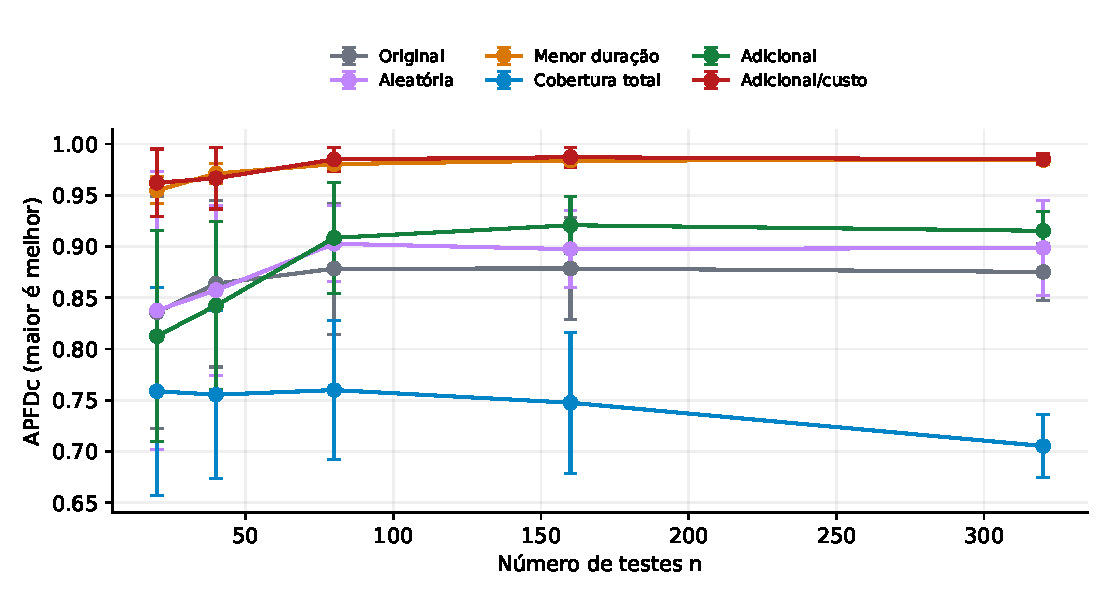
\includegraphics[width=.88\textwidth]{../figures/apfdc.pdf}
\caption{APFDc médio por tamanho. As barras representam um desvio-padrão, não intervalos de confiança.}\label{fig:apfdc}
\end{figure}

Na Figura~\ref{fig:apfdc}, o comportamento depende do tamanho da instância. Comparar tamanhos exige cautela: muda também o conjunto detectável. Em $n=320$, o número médio de defeitos detectáveis foi 17,3, e não 18 em todas as amostras. Valores de 100\% no orçamento indicam todos os defeitos detectáveis daquela instância. A conclusão sobre um algoritmo não pode ser baseada apenas em sua maior média em uma tabela.

\subsection{QP2: crescimento observado e limites teóricos}
A Figura~\ref{fig:time} mostra o tempo mediano de priorização. O ajuste exploratório $t(n)=a n^b$, por regressão linear em escala logarítmica dos cinco pontos medianos, produziu $b=1,996$ para ambos os gulosos adicionais, com $R^2>0,999$. Como $m$ permanece limitado a 40 neste objeto, o crescimento é compatível com o termo quadrático em $n$. O ajuste descreve somente o intervalo observado; não constitui prova de complexidade nem valida o comportamento quando $m$ também cresce.

\begin{figure}[ht]
\centering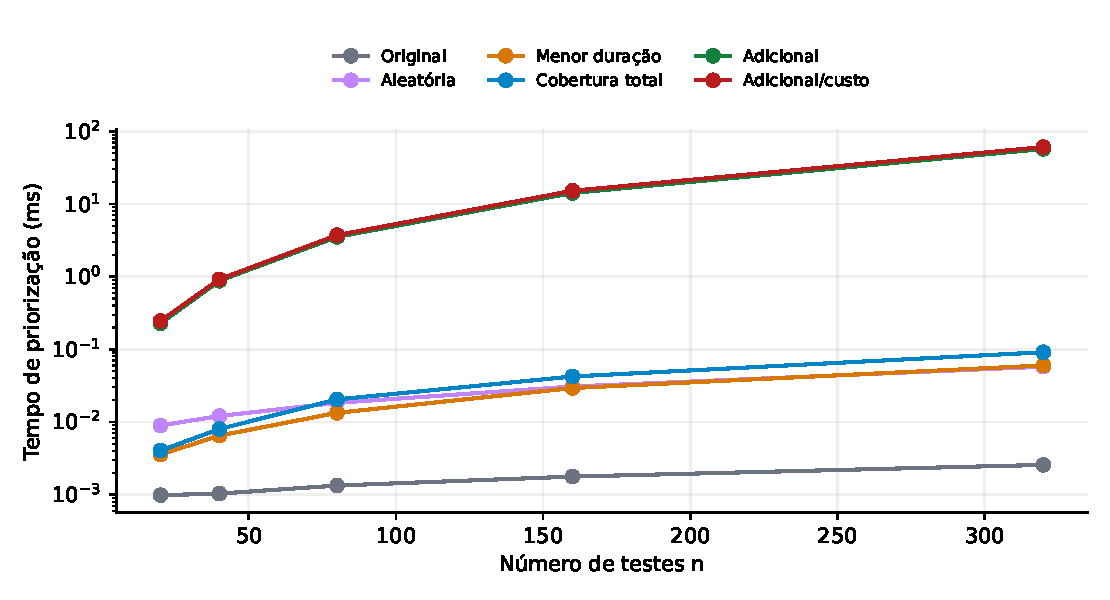
\includegraphics[width=.88\textwidth]{../figures/tempo_priorizacao.pdf}
\caption{Tempo mediano de priorização; eixo vertical logarítmico.}\label{fig:time}
\end{figure}

O número de consultas aos conjuntos, mostrado na Figura~\ref{fig:ops}, oferece evidência independente de ruído do relógio. A curva de referência $n^2$ é escalada ao primeiro ponto e serve apenas para comparar crescimento. Reinícios e tamanhos variáveis de $C_i$ alteram as constantes. Dividir pelo custo acrescenta operações, mas não muda o limite assintótico adotado.

\begin{figure}[ht]
\centering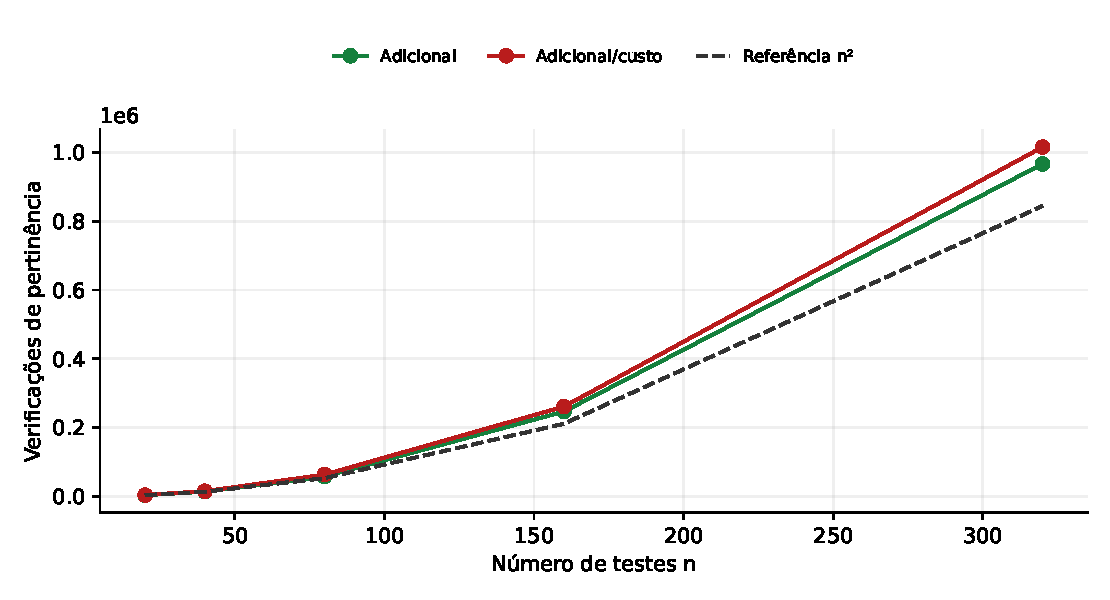
\includegraphics[width=.83\textwidth]{../figures/operacoes.pdf}
\caption{Consultas de pertinência e referência quadrática com escala ajustada.}\label{fig:ops}
\end{figure}

Os expoentes ajustados das estratégias referência, aleatória, menor duração e total foram 0,355, 0,672, 1,032 e 1,140. Os dois primeiros são inferiores ao limite linear, o que é plausível no intervalo pequeno: custos fixos de chamadas, construção do gerador aleatório e medição afetam a curva. Os próximos de um não distinguem crescimento linear de $n\log n$ nesse domínio. Não se substitui a análise do código por um expoente ajustado a cinco pontos.

O pico mediano auxiliar em $n=320$ ficou próximo de 50 KiB nos gulosos, acima dos métodos de ordenação simples. A medição não representa memória residente total, não inclui a matriz de entrada previamente alocada e não identifica sozinha uma classe assintótica. Ela complementa a derivação $O(n+m)$ e permite verificar o custo concreto da implementação.

\subsection{QP3: custo para obter feedback}
Ao somar priorização e primeira detecção, as medianas em $n=320$ foram 0,0047 ms para referência, 0,0592 ms para aleatória, 0,0601 ms para menor duração, 0,1223 ms para total, 57,2813 ms para adicional e 60,7485 ms para adicional/custo. O excelente APFDc do último não compensou seu cálculo nesse critério. Esses valores são medianas das somas por instância; não foram obtidos somando medianas independentes.

\begin{figure}[ht]
\centering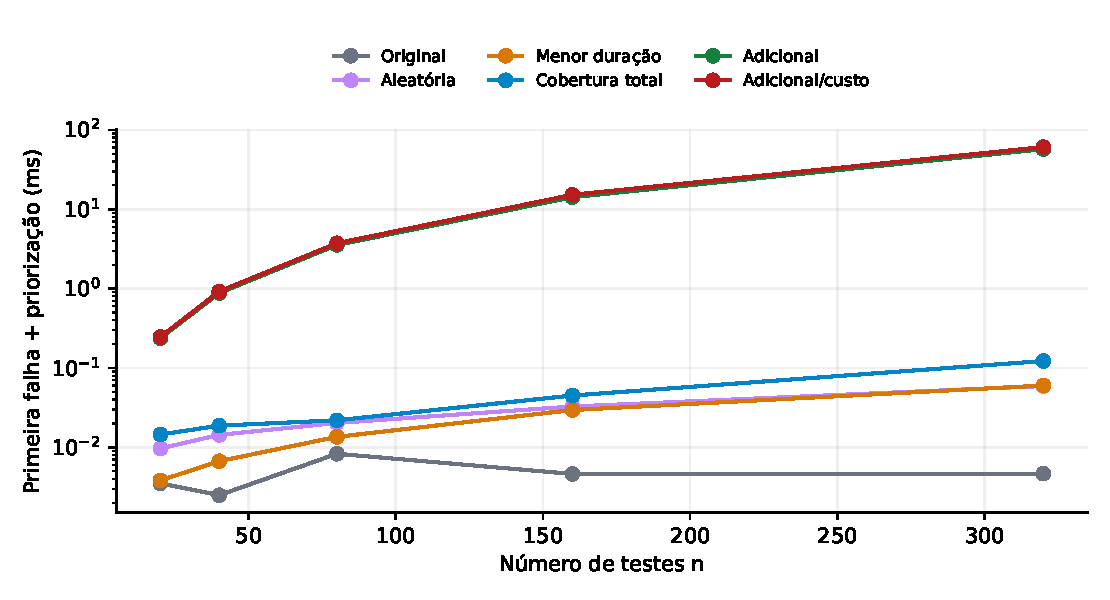
\includegraphics[width=.88\textwidth]{../figures/feedback_total.pdf}
\caption{Estimativa de tempo até o primeiro defeito, incluindo priorização.}\label{fig:feedback}
\end{figure}

O achado decorre do regime estudado: testes de funções curtas e um priorizador que recalcula ganhos repetidamente. Não significa que priorização seja dispensável em sistemas com testes demorados. O custo de coletar cobertura e durações também não entra em $P$, pois é tratado como informação anterior disponível. Cobrá-lo em cada ciclo aumentaria o custo total. Reutilização entre versões e aceleração do adicional são extensões relevantes, mas não foram avaliadas.

\subsection{Ameaças à validade}
\textbf{Construção:} os defeitos são alterações planejadas, e casos e oráculo compartilham uma especificação. Erros correlacionados entre eles são possíveis. Seis testes automatizados do método verificam exemplos de métricas, permutações, término com ganho zero e casos-base; esses controles reduzem erros de implementação, sem provar que o modelo de defeitos é representativo.

\textbf{Interna:} o ambiente compartilhado, o coletor de memória, o interpretador e a escala de microssegundos introduzem ruído. Cobertura e memória foram medidas separadamente do tempo, e lotes reduziram parte do custo fixo. Cada configuração foi repetida, mas a ordem fixa de avaliação das estratégias ainda permite efeitos de deriva do ambiente. Custos são medianas únicas reutilizadas na simulação, não novas amostras a cada permutação.

\textbf{Externa:} há somente um programa pequeno, sem banco de dados, rede, dependências de execução ou defeitos históricos. O sorteio de subconjuntos não cria dez sistemas independentes. \textbf{Conclusão:} as médias descrevem este experimento; não foram realizados testes de hipótese nem uma análise de poder. Uma avaliação industrial, com diferentes sistemas, durações e histórias de evolução, é necessária antes de recomendar uma estratégia geral.
\section{Conclusão}
A comparação preservou todos os testes de cada instância e relacionou heurísticas gulosas ao custo da implementação. No ambiente controlado, adicional/custo e menor duração apresentaram APFDc semelhante, enquanto a ordem de referência obteve o menor tempo até o primeiro defeito quando se incluiu a priorização. Assim, eficácia da ordem e custo para produzi-la respondem a questões diferentes.

O crescimento dos gulosos foi compatível com $O(n^2m)$ para $m$ limitado. Como extensões, propõem-se sistemas existentes, defeitos históricos e redução dos recálculos. O pacote inclui código e dados; os autores deverão acrescentar a URL do repositório público antes da entrega.

\paragraph{Uso de IA e estado de revisão.} Houve apoio das ferramentas de IA ChatGPT e Claude na busca e conferência de fontes, elaboração desta minuta, implementação, depuração, execução e interpretação inicial dos experimentos. Os resultados apresentados foram produzidos pelo código disponibilizado. Os autores ainda devem revisar as afirmações, realizar suas próprias leituras, repetir o experimento e assumir responsabilidade pelo texto. Os contatos dos autores aguardam confirmação.
\bibliographystyle{sbc}
\bibliography{referencias}
\end{document}
